% Overleaf: https://www.overleaf.com/4339381117cznktrnzshnt
% (The final document with the correct format is the Overleaf one)

\RequirePackage[2020-02-02]{latexrelease}
\documentclass[twocolumn]{revtex4}

\usepackage[utf8]{inputenc}
\usepackage{lmodern}
\usepackage[T1]{fontenc}
\usepackage{mathtools}
\usepackage{float}
%\usepackage{multicol}
\usepackage{csvsimple}
\providecommand{\abs}[1]{\lvert#1\rvert}
\usepackage{braket}
\providecommand{\eq}[2]{
    \begin{equation}
        #2
    \label{eq:#1}
    \end{equation}
}
\providecommand{\eqgat}[2]{
    \begin{gather}
        #2
    \label{eq:#1}
    \end{gather}
}
\usepackage{amsmath}
\usepackage{amsfonts}
\DeclareMathOperator{\calH}{\mathcal{H}}
\DeclareMathOperator{\calL}{\mathcal{L}}
\DeclareMathOperator{\calN}{\mathcal{N}}
\DeclareMathOperator{\calO}{\mathcal{O}}
\DeclareMathOperator{\tr}{tr}
\usepackage{fancyhdr}
\usepackage{wrapfig}
\usepackage{graphicx}
\usepackage[hidelinks]{hyperref}


\begin{document}


\pagestyle{fancy}
\lhead{\bf Entanglement Entropy and Holography}
\rhead{Ferran Rodríguez Mascaró}
\lfoot{Treball de Fi de Grau}
\rfoot{Barcelona, January 2023}


\title{Entanglement Entropy and Holography}
\author{Author: Ferran Rodríguez Mascaró}
\email{ferran.r.m11@gmail.com} %optional
\affiliation{Facultat de F\'{\i}sica, Universitat de Barcelona, Diagonal 645, 08028 Barcelona, Spain.}
\author{Advisor: Dr. Pablo Bueno Gómez}
%\date{\today}


\begin{abstract}
    {\bf Abstract:} The AdS/CFT correspondence, also called \emph{holography}, is a physical duality between quantum gravity theories in anti-de Sitter (AdS) spacetimes and certain quantum field theories (QFTs) with conformal symmetry defined in the boundary of such space. The so-called holographic dictionary describes how quantities from each of these theories can be translated into quantities of the other. An important magnitude of the holographic dictionary is the entanglement entropy (EE) of boundary regions. This measures the degree of quantum entanglement between such regions and their complements. In this work, we study various aspects of EE in the holographic context. After a quick review of AdS/CFT and of general aspects of EE in QFT, we introduce the Ryu-Takayanagi formula, which computes the holographic EE of boundary regions in the semiclassical limit of the gravity side of the duality. We perform explicit calculations and general checks of the formula, review its generalizations to account for stringy and quantum corrections, and comment on its relation with black hole thermodynamics and the emergence of gravitational dynamics.
\end{abstract}


\maketitle


\section{Introduction} \label{s:Intro}
The search for a unification of quantum theories and gravity is a long-standing challenge in theoretical physics. The AdS/CFT correspondence ---appeared in the late 1990s in the context of string theory \cite{maldacena_large_1999}--- provides such unification in the particular case of spacetimes with a timelike boundary. AdS/CFT is also a realization of the holographic principle, which establishes that quantum gravity theories must admit an equivalent description in terms of theories which live at the boundary of the corresponding spacetimes.  % as a breakthrough in the research on the fundamental principles that govern our universe.
In addition to its fundamental implications in the search for an ultimate theory of all the interactions, AdS/CFT provides a useful framework for proving aspects of quantum field theories (QFTs) in regimes in which the usual tools cannot be applied ---{\emph e.g.,} when the fields are strongly coupled--- using the tools of classical general relativity. %For 
%In traditional quantum field theories, gravity is not directly incorporated into the framework, and the gravitational force is typically treated classically. However, 
Additionally, AdS/CFT allows us to study the quantum behavior of gravity by relating it to well-defined and well-understood QFTs.
In this work we study an example of the first class of applications, namely, how the quantum entanglement of region algebras in holographic QFTs is encoded in a completely classical quantity from the gravity side.

%One of the main motivations behind it is to better understand the behavior of strongly coupled quantum field theories, which are notoriously difficult to study. AdS/CFT provides a powerful tool to explore the dynamics of such systems by mapping them to classical gravitational theories in AdS spaces.

%AdS/CFT reveals that the entanglement structure of a quantum field theory corresponds to the gravitational interactions and curvature of AdS. The spacetime geometry emergence from entanglement becomes evident.
In section \ref{s:Holo_AdS/CFT} we introduce the holographic principle and the AdS/CFT correspondence. The notion of entanglement entropy (EE) and some of its properties ---including a generalization of the first-law of thermodynamics--- in the context of conformal field theories (CFTs) is presented in section \ref{s:EE_CFT}. In section \ref{s:EE_Holo} we introduce the Ryu-Takayanagi formula, which allows to compute the holographic EE of boundary regions from the area of extremal surfaces in anti-de Sitter (AdS) space. We evaluate the EE in the case of a circular region in CFT$_3$ explicitly and verify that the prescription fulfills the fundamental property of {\it strong subadditivity}. In section \ref{s:EE_Holo} we provide an overview of how the Ryu-Takayangi formula gets corrected by stringy and quantum effects. 


\section{Holography and AdS/CFT} \label{s:Holo_AdS/CFT}


\subsection{The Holographic Principle} \label{ss:Holography}

Given a finite space region, imagine a process in which matter is continuously added into it. This will make the entropy increase. However, there is a limit to the amount of matter that can be introduced in the region, corresponding to the moment in which a black hole is formed. The entropy of a black hole only depends on its surface area and is given, in Planck units, by \cite{bekenstein_black_1973, hawking_particle_1975}
\eq{BH}{
    S_\text{BH} = \frac{ A_\text{H} }{ 4 G } \ ,
}
where $A_\text{H}$ is the area of the event horizon of the black hole and $G$ is Newton's gravitational constant. As a consequence, the maximum entropy that a region can contain is given by its area divided by $4G$.

This implies that the degrees of freedom inside some region grow with the area of the boundary and not with the volume of the region, as one might have expected. This leads to the \emph{holographic principle}, which states that in a quantum gravity theory all physics phenomena within some volume must be describable in terms of a theory defined on the boundary of the region \cite{t_hooft_dimensional_2009}.


\subsection{AdS/CFT Correspondence} \label{ss:AdS/CFT}

The \emph{AdS/CFT correspondence}, sometimes simply called \emph{holography} or \emph{gauge/gravity correspondence} \cite{maldacena_large_1999}, is an explicit realization of the holographic principle. It establishes the complete physical equivalence between quantum gravity theories living in anti-de Sitter spacetimes and certain types of CFTs living in the boundary of such spacetimes. If the gravitational theory is defined in $(d+1)$ spacetime dimensions, the dual CFT is defined in $d$ spacetime dimensions and, in a precise sense, the gravity theory will be a ``hologram'' of the CFT. AdS/CFT allows us to study aspects of each of these theories through the other. The so-called \emph{holographic dictionary} maps quantities (observables) between the gravity theories and their dual CFTs \cite{witten_anti_1998}. For example, an empty AdS spacetime with no matter is dual to the vacuum state of the CFT, and an AdS spacetime with a black hole inside corresponds to a thermal state in the CFT.

An anti-de Sitter spacetime is a maximally symmetric spacetime with negative curvature, which solves Einstein's field equations with a negative cosmological constant. The metric of an AdS spacetime of $(d+1)$ dimensions in Poincar\'e coordinates is 
\eq{AdS_PP-metric}{
    \mathrm{d} s_{\text{AdS}_{(d+1)}}^2 = \frac{L^2}{z^2} \left( -\mathrm{d} t^2 + \mathrm{d} z^2 + \sum_{i=1}^{d-1} \mathrm{d} x_i^2 \right) \ ,
}
with the time and spatial dimensions $t , x_i \in (-\infty,+\infty)$, an extra dimension $z \in (0,+\infty)$, sometimes called \emph{holographic coordinate}, and where $L$ is the \emph{AdS radius}. Fixing the coordinate $z$, the metric reduces to the one of $d$-dimensional Minkowski spacetime ``weighted'' by the constant factor $1/z^2$. Hence, AdS can be foliated by Minkowski spacetimes living at different values of $z$.

% La citación a Kaplan no funciona. ¿Referencia para AdS en Poincaré patch?

\begin{wrapfigure}[13]{r}{0.25\textwidth}
    \centering
    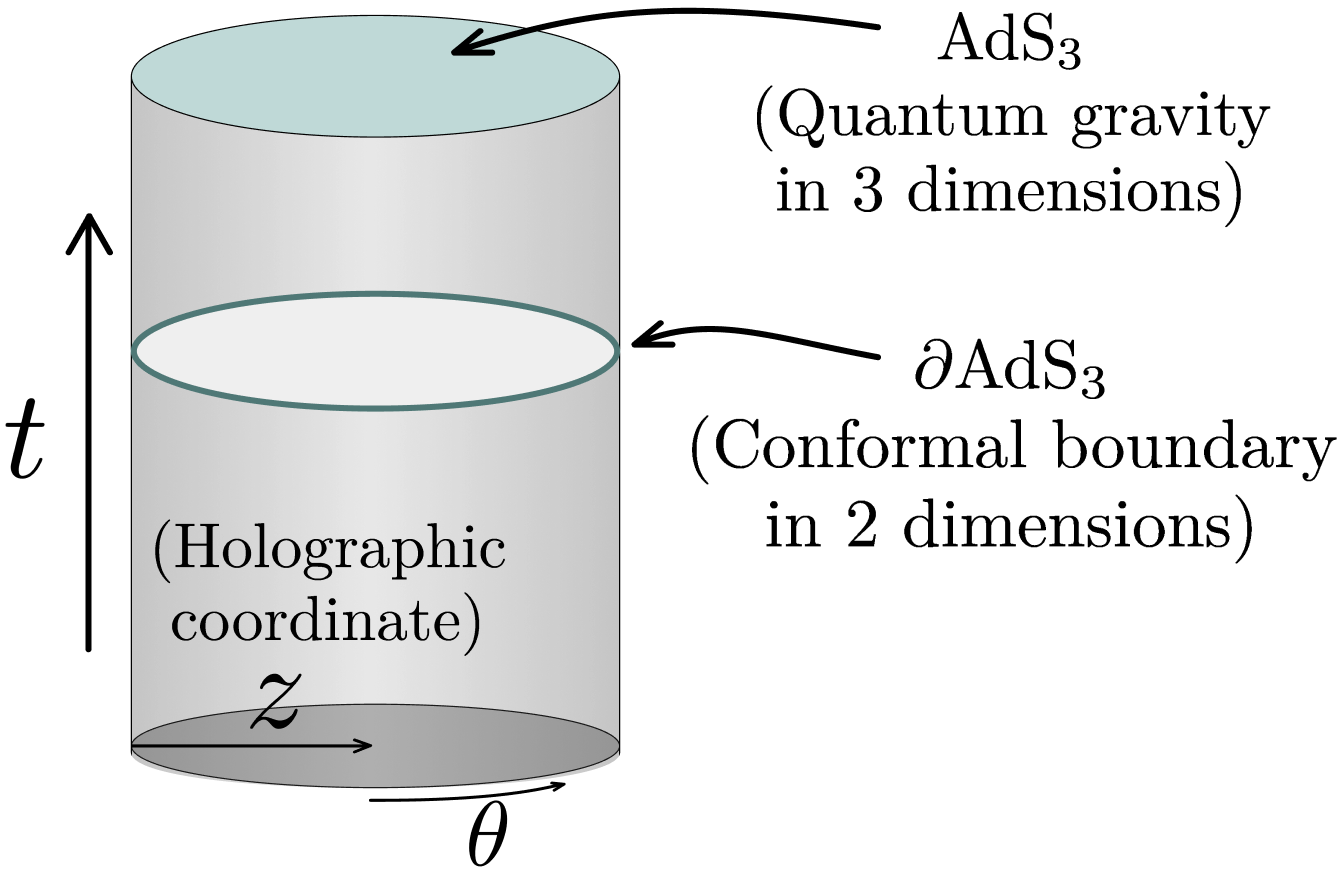
\includegraphics[width=0.25\textwidth]{../imatges/AdS_Cylindric.png}
\caption{AdS$_3$ spacetime. In the conformal boundary lives the CFT$_2$.}
\label{fig:AdS}
\end{wrapfigure}

AdS$_{d+1}$ can be represented as a cylinder where each slice corresponds to a constant time and where  $z$ grows radially towards the center \cite{hawking_large_2008}. Each slice has a $d$-dimensional boundary $\partial$AdS$_{(d+1)}$ where the CFT$_d$ lives (Fig.~\ref{fig:AdS}).

CFTs, on the other hand, are QFTs that are invariant under conformal transformations. These are angle-preserving transformations which leave the metric invariant up to an overall factor \cite{di_francesco_conformal_1997}. The Poincar\'e group is a subgroup of the conformal group, but there are additional transformations corresponding to dilatations and special conformal transformations. The number of generators of a $d$-dimensional CFT coincides with the number of isometries of a $(d+1)$-dimensional AdS spacetime. This is a hint of the holographic duality.

The first instance of the AdS/CFT correspondence ever described was the duality between $d=4$, $\calN=4$ Super Yang-Mills theory and type-IIB string theory on AdS$_5 \times $S$_5$ \cite{maldacena_large_1999}, but many other examples are known by now. Many general rules of the duality can be exploited without specifying the full field content of the theories and here we will make use of this fact.

AdS/CFT is valid independently of the intensity of the gravitational coupling. Interestingly, a strongly coupled CFT with a large number of colors is dual to a classical gravitational theory. %As it will be seen shortly,
In this situation, it is possible to explain classical gravitational phenomena by highly quantum features, and vice versa, using the holographic dictionary.


\section{Entanglement Entropy in CFT} \label{s:EE_CFT}

Given some quantum system composed of two subsystems $A$ and $B$ in a pure state $\ket{\Psi}$, there are two possibilities. If one can write $\ket{\Psi}$ as a single tensor product of pure states, $\ket{\Psi} = \ket{\Phi}_A \otimes \ket{\tilde{\Phi}}_B$, one say that the state is separable. If this is not possible, $\ket{\Psi} \neq \ket{\Phi}_A \otimes \ket{\tilde{\Phi}}_B$, one say that the state is entangled.
%of a system, two subsystems $A$ and $B$ that divides this system will be separable if it is possible define the state $\ket{\Psi}$ as a combination of one individual state for each subsystem ($\ket{\Psi} = \ket{\Phi}_A \otimes \ket{\tilde{\Phi}}_B$), and \emph{entanglet} if it is not ($\ket{\Psi} \neq \ket{\Phi}_A \otimes \ket{\tilde{\Phi}}_B$) -~see e.g., \cite{schrodinger_discussion_1935}. 
In the latter case, one cannot describe neither of them independently without losing information (in other words, if one trace over one of the subsystems, the reduced state of the other will not be pure). The two form an inseparable entity.

The \emph{entanglement entropy} (EE) is a measure of the degree of quantum entanglement between two subsystems \cite{nishioka_entanglement_2018}. It is defined by the von Neumann entropy of the reduced density matrix $\rho_A$ of one of the subsystems as
\eq{EE}{
    S(A) \equiv - \tr_A ( \rho_A \log \rho_A ) \ ,
}
being $\rho_A = \tr_B \ket{\Psi}\bra{\Psi}$. If $\lambda_i$ are the eigenvalues of $\rho_A$, then the entanglement entropy would take the simplified form $S = - \sum_i \lambda_i \log \lambda_i$. The von Neumann entropy is always positive, and is zero for a pure state, so that the EE of separable states vanishes, as it should. 


The natural subsystems in QFT are spacetime regions. For any QFT, given a global state and some region $A$, there is a regulated sense in which it induces a density matrix $\rho_A$ from which one can compute its EE with respect to its causal complement.
%For a QFT living in Minkowski spacetime, one can define operator algebras that define spacetime regions. Discretizing the lattice, a density matrix is associated to the region that only depends on its algebra and its surroundings. From this density matrix, an entanglement entropy can be defined. 
This EE is intrinsically divergent, since the region is separated from its vicinity by a zero-dimensional boundary. Nonetheless, one can regulate it and obtain physically meaningful results.

The general expression of the EE for an arbitrary region in a $d$-dimensional CFT is ---see {\emph{e.g.,}} \cite{nishioka_entanglement_2018},
\begin{gather}
    S_A^{\text{CFT}_d} = c_{d-2} \left( \frac{H}{\delta} \right) ^{d-2} + c_{d-1} \left( \frac{H}{\delta} \right) ^{d-4} + \dots \label{eq:EE_CFT} \\
    + \begin{dcases}
        c_1 \frac{H}{\delta} + (-1)^{\frac{d-1}{2}} s_{\text{univ}}
        \qquad \qquad \qquad \quad \ \text{for odd } d \, , \\
        c_2  \frac{H}{\delta} + (-1)^{\frac{d-2}{2}} s_{\text{univ}} \log \left ( \frac{H}{\delta} \right ) + c_0
        \quad \text{for even } d \, ,
    \end{dcases} \nonumber
\end{gather}
where $H$ is the characteristic length of region $A$, $\delta$ is an ultraviolet cut-off, $c_i$ are coefficients that are non-universal (not well-defined in the continuum, i.e., dependent on the definition of $\delta$), and $s_{\text{univ}}$ are universal coefficients that contain well-defined (``universal'') information about the corresponding QFT.


\subsection{The first law of entanglement entropy}
The EE satisfies an interesting relation known as the 
\emph{first law of entanglement entropy}. %is an important direct outcome of the definition of the EE (Eq.~\ref{eq:EE}) 
Here we derive it and show that it incorporates the usual first-law of thermodynamics as a particular case.

Consider a family of states $\ket{\Psi(\lambda)}$ defined by the parameter $\lambda$ of a general quantum system with a subsystem $A$. The first order variation of the EE is \cite{van_raamsdonk_lectures_2017}
\eqgat{varEE}{
    \frac{\mathrm{d}}{\mathrm{d} \lambda} S_A %= - \frac{\mathrm{d}}{\mathrm{d} \lambda} (\rho_A \log \rho_A) = \nonumber \\
    = - \tr \left( \log \rho_A \frac{\mathrm{d}}{\mathrm{d} \lambda} \rho_A \right) - \tr \left( \frac{\mathrm{d}}{\mathrm{d} \lambda} \rho_A \right) \ ,
}
where the last term vanishes since the trace of the density matrix is one for any state.

Now, given any state $\rho$, its \emph{modular Hamiltonian} is defined as $H = - \log \rho$. %, related to the density matrix with no perturbation $\rho_A (\lambda=0)$.
Using this, the last equation can be rewritten  as
\eq{1law}{
    \frac{\mathrm{d}}{\mathrm{d} \lambda} S_A = \frac{\mathrm{d}}{\mathrm{d} \lambda} \braket{H_A} \ ,
}
where $\braket{H_A} \equiv \tr (H_A \rho_A)$ is the expectation value of the modular Hamiltonian of $\rho_A$ in the same state. This is the first law of EE. It %is called like this because it 
represents a quantum generalization of the first law of thermodynamics, which can be seen by considering the case where the unperturbed density matrix is in a  thermal state. In that case, the modular Hamiltonian is related to the usual Hamiltonian of the system $H$ by
$
    \rho_A =  e^{-H/T} 
$, where $T$ is the temperature,
and the EE becomes a thermal entropy. Applying Eq.~\ref{eq:1law} and the definition of the modular Hamiltonian, it is immediate to obtain that, in this case,
\eq{1law_thermo}{
    \frac{\mathrm{d}\braket{H}}{\mathrm{d} \lambda}  =  T \frac{\mathrm{d}S_A}{\mathrm{d} \lambda}  \ .
}
In other words, $\mathrm{d} E = T \, \mathrm{d} S$. Therefore, we see that the usual first law of thermodynamics is a consequence of  the more fundamental first law of EE.


\section{Holographic Entanglement Entropy} \label{s:EE_Holo}


\subsection{Ryu-Takayanagi formula} \label{ss:R-T}

For general CFTs, it is very difficult to compute the EE of a region. On the other hand, it turns out to be rather easy to do it for holographic CFTs. Remarkably, in the holographic context, an essentially quantum quantity such as EE can be obtained from areas of extremal surfaces on AdS spacetime.

Given a gravity theory defined on ($d+1$)-dimensional AdS spacetime, the dual CFT will live at its conformal boundary. This is a $d$-dimensional Minkowski space, which lies, in Poincar\'e coordinates, at 
%given a region $A$ in its boundary $d$-dimensional Minkowski spacetime slice formed from fixing $z$ as 
$z=\delta \ll 1$. The EE for a region $A$ in the holographic CFT can be computed using the so-called Ryu-Takayanagi formula \cite{ryu_holographic_2008}:
\eq{EE_RT}{
    S_A = \frac{ \text{Area}(\gamma_A^\text{min}) }{ 4 G } \ ,
}
where $\gamma_A^\text{min}$ is the surface of minimal area defined on AdS spacetime connected to the ($d-1$)-dimensional boundary $\partial A$ of the region $A$, and $G$ is the ($d+1$)-dimensional Newton constant ---see Fig.~\ref{fig:EE_AdS-CFT}.

The area of $\gamma_A^\text{min}$ is obtained by
\eq{EE_RT-area}{
    \text{Area}(\gamma_A^\text{min}) = \int_{\gamma_A} \sqrt{h} \ \mathrm{d}^{d}y \ ,
}
where $y$ are the $d$ coordinates that represent the surface $\gamma_A^\text{min}$ and $h$ is the determinant of the metric $h_{ij} = (\partial x^\mu / \partial y^i) (\partial x^\nu / \partial y^j) \, g_{\mu\nu}$ induced on the surface by the surrounding spacetime.

\begin{wrapfigure}[14]{r}{0.25\textwidth}
    \centering
    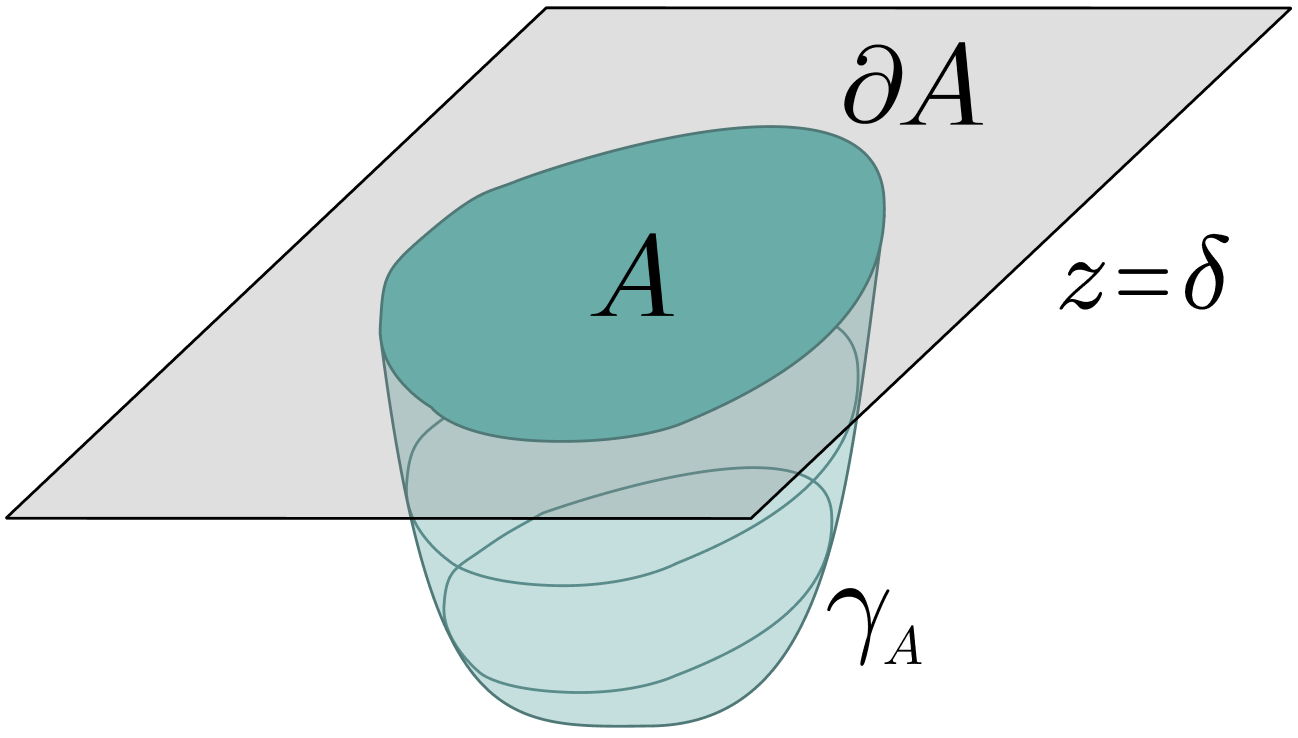
\includegraphics[width=0.25\textwidth]{../imatges/EE_AdS-CFT-D.png}
\caption{Region $A$ (dark blue) and its boundary $\partial A$ inside a $z=\delta$ AdS slide (grey) and its respective $\gamma_A$ (light blue) inside the AdS spacetime.}
\label{fig:EE_AdS-CFT}
\end{wrapfigure}

The Ryu-Takayanagi formula is valid for generic systems, and provides a hint on how the geometry of spacetime can emerge from mere quantum information.

As one can verify, the Ryu-Takayanagi formula for a ($d+1$)-dimensional anti-de Sitter reproduces the expected general behaviour of the EE (Eq.~\ref{eq:EE_CFT}) for a $d$-dimensional conformal field theory \cite{ryu_aspects_2006, nishioka_holographic_2009}. Let us see this explicitly.


\subsection{Entanglement Entropy for a Disk in CFT\texorpdfstring{$_3$}{3}} \label{ss:EE-disk}

In this section, we compute the EE for a circular region in a holographic CFT$_3$ dual to Einstein gravity. We will use this calculation to verify the general expression of the EE for a QFT, identify the universal coefficient for this kind of theory, and illustrate how AdS provides us with a geometric ultraviolet regulator.

Let $A$ be a disk-shaped region of radius $R$ defined in the conformal boundary of pure AdS$_4$. This region is defined in polar coordinates as
$
    A = \{ ( r, \theta, z, t ) \ | \ t = 0, z = \delta, r \le R \} 
$. 
We parameterize the minimal area bulk surface as:
$
    \gamma_A^\text{min} = \{ ( r, \theta, z, t ) \ | \ t = 0, z = f (r, \theta) \} %\ , \nonumber
$, 
where $f(r,\theta)$ is certain function we need to identify. There is no property on the AdS spacetime theory that could prevent the symmetry of $\partial A$ on the coordinate $\theta$ from being transferred to $\gamma_A^\text{min}$. Hence, $z=f(r)$.
The AdS$_4$ metric reads
\eq{1Ametric}{
    \mathrm{d}s^2_{\text{AdS}_4} = g_{\mu \nu} \mathrm{d}x^\mu \mathrm{d}x^\nu = 
    \frac{L^2}{z^2} [ -\mathrm{d}t^2 + \mathrm{d}z^2 + \mathrm{d}r^2 + r^2 \mathrm{d}\theta^2 ] \ . \nonumber
}
The induced metric of the surface $\gamma_A^\text{min}$ is in turn given by
\eq{1gammaAmetric}{
    \mathrm{d}s^2_{\gamma_A^\text{min}} = h_{i j} \mathrm{d}x^i \mathrm{d}x^j = 
    \frac{L^2}{f(r)^2} \left[ \left( 1+ \dot{f}(r)^2 \right) \mathrm{d}r^2 + r^2 \mathrm{d}\theta^2 \right] \ , \nonumber
}
where $ \dot{f}(r) \equiv \partial f/\partial r$. The determinant of the induced metric will be
$
    h = L^4 r^2 ( 1 + \dot{f}(r)^2 )/f(r)^4 
$.  
The minimal value of the integral over the polar coordinates of the square root of the induced metric will correspond to the area of $\gamma_A^\text{min}$. So, by the Ryu-Takayanagi formula, the EE related to the region $A$ will be
\eq{1EEA}{
    S_A = \text{min} \int_{\gamma_A}    \frac{\sqrt{h} \ \mathrm{d}x^\rho}{4G} = \frac{\pi L^2}{2G} \, \text{min} \int_r \mathrm{d}r \frac{r \sqrt{ 1 + \dot{f}(r)^2 }}{f(r)^2}  \ ,\nonumber
}
where in the second line we performed the angular integration. The resulting integral in $r$ must be evaluated on the minimal surface. In order to find it, we extremize the functional using the 
%The interior of this final definite integral looks like some type of Lagrangian , whose 
Euler-Lagrange equations for the effective Lagrangian $\calL [r,f(r),\dot{f}(r)]$. They read
\eqgat{1EL}{
    \frac{\partial \calL}{\partial f} - \frac{\mathrm{d}}{\mathrm{d}r} \left[ \frac{\partial \calL}{\partial \dot{f}} \right] = 0 \nonumber \\
    \longrightarrow \left( 1+\dot{f}^2 \right) \left( -2r-f\dot{f}-rf\ddot{f} \right) + rf\dot{f}^2\ddot{f} = 0 \ .\nonumber
}
One can prove that $f(r) = \sqrt{R^2 - r^2}$ is a solution of the previous relation and corresponds to the function that minimizes the functional of the EE and connects to the boundary region $A$. Hence, the surface of minimal area is found to be a half sphere.

To compute the integral of the EE expression, we should first determine its limits carefully. The inferior one corresponds to the lower part of the half sphere inside the bulk, where $r_\text{min}=0$. The superior one connects the surface with the conformal boundary, that is, $z=\delta=\sqrt{R^2-r_\text{max}^2}$. Had we not included $\delta$ and had integrated all the way to $z=0$, the result would have diverged. This is precisely what we expect for the EE, which becomes divergent in the continuum. In this case, the geometric cutoff introduced in the holographic coordinate, $z=\delta$, plays the role of the ultraviolet regulator of the EE. The final result for the EE of the disk is 
\eqgat{1sol}{
    S_A = \frac{\pi L^2}{2G} \, \int_0^{\sqrt{R^2-\delta^2}} \mathrm{d}r \frac{r}{f(r)^2} \sqrt{ 1 + \dot{f}(r)^2 } = \nonumber \\
    = \frac{\pi L^2}{2G} \frac{R}{\delta} - \frac{\pi L^2}{2G}+\mathcal{O}(\delta) \ . \nonumber
}
This coincides with the general expression expected for the EE of  a 3-dimensional CFT. Repeating the calculation for various regions and in different dimensions, the corresponding structure found is always consistent \cite{ryu_aspects_2006,ryu_holographic_2008}. 

From the above expression we can identify the universal contribution to the EE for a 3-dimensional holographic theory dual to Einstein gravity. The result reads
\eq{suniv}{
     s_\text{univ} = \frac{\pi}{2} \frac{L^2}{G} \ .
}

In the case of a disk region, like the one we just considered, $s_\text{univ}$ is related to another important quantity, namely, the Euclidean free energy on a three-dimensional sphere. One has $s_\text{univ}= -\log Z_{\mathbb{S}^3}$ for general CFTs \cite{casini_towards_2011}. Hence, we find that for holographic theories dual to four-dimensional Einstein gravity, the sphere free energy is given in terms of the AdS radius and the Newton constant by (\ref{eq:suniv}).
% He puesto la cite the Casini,2011. Entiendo que es esta.


\subsection{Strong subadditivity} \label{ss:SS}

\emph{Strong subadditivity}  is a fundamental general property of EE. It relates the EEs of two regions $A$ and $B$ with the ones of their union $A \cup B$ and intersection $A \cap B$ %, and relative complements $A \setminus B$ and $B \setminus A$ 
(Fig.~\ref{fig:SS}):
\eqgat{EE_strong-subadd}{
    S(A) + S(B) \ge S(A \cup B) + S(A \cap B) \ . %\nonumber \\
    %S(A) + S(B) \ge S(A \setminus B) + S(B \setminus A) \ .
}
\begin{wrapfigure}[13]{r}{0.25\textwidth}
    \centering
    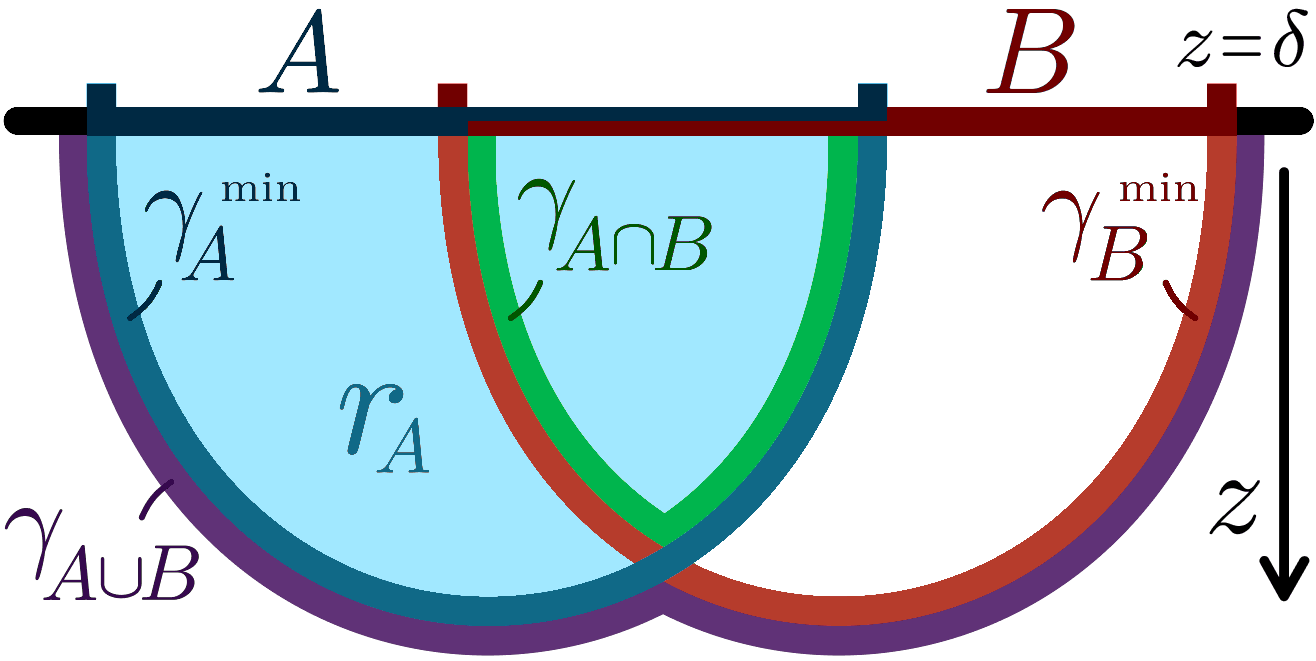
\includegraphics[width=0.25\textwidth]{../imatges/SS_2-D.png}
\caption{Representation of the surfaces $\gamma_A^\text{min}$ and $\gamma_B^\text{min}$, their union $\gamma_{A \cup B}$ and intersection $\gamma_{A \cap B}$, and the bulk region $r_A$.}
\label{fig:SS}
\end{wrapfigure}
This inequality is fulfilled in any quantum mechanical theory, but it is remarkably difficult to prove in general. An important test of the validity of the Ryu-Takayanagi formula is whether it fulfills it. It turns out to be particularly easy to prove that it does \cite{headrick_holographic_2007}.

We define $r_A$ and $r_B$ to be the bulk regions inside $\gamma^{\text{min}}_A$ and $\gamma^{\text{min}}_B$, respectively. Their union and intersection will be $r_{A \cup B} \equiv  r_A \cup r_B$ and $r_{A \cap B} \equiv  r_A \cap r_B$. The boundaries of these regions can be decomposed as
\eq{SS_dr-1}{
    \partial r_{A \cup B} = (A \cup B) \cup \gamma_{A \cup B} \ , \ \partial r_{A \cap B } = (A \cap B) \cup \gamma_{A \cap B} \ , \nonumber
}
where $\gamma_{A \cup B}$ and $\gamma_{A \cap B}$ are the segments inside the bulk of the boundary surfaces of $r_{A \cup B}$ and $r_{A \cap B}$. These surfaces are connected to $\partial (A \cup B)$ and $\partial (A \cap B)$, respectively, but nothing says that they should be their corresponding minimal area surfaces $\gamma^{\text{min}}_{A \cup B}$ and $\gamma^{\text{min}}_{A \cap B}$. The areas of $\gamma_{A \cup B}$ and $\gamma_{A \cap B}$ correspond to upper bounds for the minimal possible area. Also, observe that the sum of the areas of $\gamma_{A \cup B}$ and $\gamma_{A \cap B}$ trivially equals the sum of the areas of $\gamma^{\text{min}}_A$ and $\gamma^{\text{min}}_B$. Hence,
\eq{SS_gamma-1}{
    {\text{Area}}(\gamma^{\text{min}}_A) + {\text{Area}}(\gamma^{\text{min}}_B) %= {\text{Area}}(\gamma_{A \cup B}) + \gamma_{A \cap B}
    \ge   {\text{Area}}(\gamma^{\text{min}}_{A \cup B}) +   {\text{Area}}(\gamma^{\text{min}}_{A \cap B}) \ . \nonumber
}
% \gamma són las superficies, no las áreas de las superficies. ¿Esta ecuación sigue siendo correcta? ¿Hay un exceso de uso de notación? En Headrick,2007 lo ponen así.
Therefore, the Ryu-Takayanagi formula (Eq.~\ref{eq:EE_RT}) implements the strong subadditivity property in a simple geometric way which makes use of the minimization principle of AdS holographic surfaces. %we proved the first inequality of Eq.~\ref{eq:EE_strong-subadd}.

%Regarding the second inequality, let's define the bulk regions exclusive of $A$ and $B$: $r_{A \setminus B}$ and $r_{B \setminus A}$, respectively. The boundary surfaces of this regions will be decomposed as
%\eq{SS_dr-2}{
%    \partial r_{A \setminus B} = (A \setminus B) \cup \gamma_{A \setminus B} \ , \ \partial r_{B \setminus A } = (B \setminus A) \cup \gamma_{B \setminus A} \ . \nonumber
%}
%Again, it is clear that the areas of $\gamma_{A \setminus B}$ and $\gamma_{B \setminus A}$ correspond to upper bounds. Hence,
%\eq{SS_gamma-2}{
%    \gamma_A + \gamma_B = \gamma_{A \setminus B} + \gamma_{B \setminus A} \ge \gamma^{\text{min}}_{A \setminus B} + \gamma^{\text{min}}_{B \setminus A} \ , \nonumber
%}
%and the second inequality of Eq.~\ref{eq:EE_strong-subadd} is proven.

%Using these simple geometric proofs, we showed how holography fulfills the strong subadditivity property that should be true in any quantum mechanical many-body system, playing the extra dimension in the holographic dual an essential role.

% Hay algunas de las pequeñas fórmulas dentro del texto que se cortan con los saltos de línea.

%\clearpage
\subsection{Corrections to the Ryu-Takayanagi formula} \label{ss:EE_HO}

The Ryu-Takayanagi formula (\ref{eq:EE_RT}) provides the EE for holographic theories dual to Einstein gravity in general dimensions. Nevertheless, the Einsteinian description breaks down if one moves away from the strongly coupled and large-number of colors regime. From the gravity side, this is manifest in the appearance of both stringy and quantum corrections. %to classical Einstein gravity.

Stringy corrections appear as higher-curvature terms in the gravity action. These produce corrections to the Ryu-Takayanagi area formula in a way similar to 
%For stringy corrections, the area functional needs to be modified, similarly to 
how the Bekenstein-Hawking formula for the entropy of a black hole (\ref{eq:BH}) is replaced by the Wald formula \cite{iyer_properties_1994} in the presence of higher-curvature corrections. However, replacing the functional of the EE by the Wald one does not work in general. The full formula takes the schematic form \cite{dong_holographic_2014}
\begin{equation}\label{hee}
    S_A=S_{\text{Wald}}+ S_{\text{Anomaly}} \ ,
\end{equation}
where $S_{\text{Wald}}$ reduces to the Ryu-Takayanagi one in the Einstein gravity case, but otherwise contains terms involving various components of the Riemann tensor, and $S_{\text{Anomaly}}$ simply vanishes for Einstein gravity, but includes terms involving extrinsic curvatures of the generalized minimal surface for more general theories. %For instance, consider a quadratic theory of the form {\bf [[[[ Poner explícitamente la fórmula para gravedad cuadrática]]]]}
%\begin{equation}
%    \mathcal{L}= \frac{1}{16\pi G}\left[\frac{6}{\ell^ 2}+R+\ell^2 \left(\alpha_1 R^ 2 + \alpha_2 R_{\mu\nu} R^{\mu\nu}\right) \right]\, ,
%\end{equation}
%where $\alpha_{1,2}$ are dimensionless couplings and $\ell^2$ coincides with the AdS radius in the Einstein gravity limit.
%The modified holographic EE formula for this theory is given by (\ref{hee}), where
%\begin{align}
%    S_{\text{Wald}}&= \, , \\
%    S_{\text{Anomaly}}&=
%\end{align}


%Additional ``anomaly'' terms corresponding to extrinsic curvatures of the generalized surface involving arbitrary contractions of Riemann tensors and metrics are required . In the anomaly term, each of the Riemann tensor components resulting has to be split into summatories of different weighted terms. The way that these terms are weighted is non-unique, leading to the so-called \emph{splitting problem}.

%\clearpage
One can also consider quantum corrections to the Ryu-Takayanagi formula related to quantum mechanical effects in the bulk. This quantum corrections are essentially given by the EE of quantum fields living inside the bulk region bounded by the minimal area surface, $r_A$ ---see Fig.~\ref{fig:SS}. The corrected formula reads \cite{faulkner_quantum_2013}
\eq{EEquantum}{
    S_A = \frac{\text{Area} (\gamma_A^\text{min})}{4 G} + S_{r_A} + \calO(G) \ ,
}
where the correction $S_{r_A}$ is order $\calO(G^0)$ and we have also included a putative subleading correction.


%\vspace{20px}
\section{Conclusions} \label{s:Conclusions}
We have explored various aspects of the Ryu-Takayanagi formula ---a summary of the results presented can be found in the introduction. This is a remarkable entry in the holographic dictionary which allows to compute a genuinely quantum quantity like the EE of boundary regions, in terms of a fully classical quantity related to the geometry of spacetime, namely, the area of extremal surfaces in AdS. The connection between spacetime geometry and entanglement can be made more explicit. Remarkably, one can show that the first law of EE implies, for holographic CFTs, that perturbations of the bulk metric satisfy the linearized Einstein equations \cite{faulkner_gravitation_2014}. In a sense, the entanglement structure of the boundary theory controls the dynamics of the gravitational field, which therefore becomes an emergent phenomenon.  



\begin{acknowledgments}

    I would like to extend my sincere gratitude to Prof. Pablo Bueno for his guidance and expertise. Also, I wish to thank my family and friends for their support and unwavering patience.
    
\end{acknowledgments}



\bibliography{TFG.bib}
% \bibliographystyle{abbrv}


\end{document}